%% LyX 2.3.2 created this file.  For more info, see http://www.lyx.org/.
%% Do not edit unless you really know what you are doing.
\documentclass[spanish,twocolumn]{bmcart}
\usepackage[utf8]{inputenc}
\setcounter{secnumdepth}{3}
\setcounter{tocdepth}{3}
\setlength{\parskip}{\smallskipamount}
\setlength{\parindent}{0pt}
\usepackage{color}

\makeatletter

%%%%%%%%%%%%%%%%%%%%%%%%%%%%%% LyX specific LaTeX commands.
%% Because html converters don't know tabularnewline
\providecommand{\tabularnewline}{\\}

%%%%%%%%%%%%%%%%%%%%%%%%%%%%%% User specified LaTeX commands.
%% BioMed_Central_Tex_Template_v1.06
\usepackage[T1]{fontenc}
%\usepackage{lmodern}
\usepackage{charter}

%\usepackage[draft]{graphicx}

%%  If you wish to display your graphics for   %%
%%  your own use using includegraphic or       %%
%%  includegraphics, then comment out the      %%
%%  following two lines of code.               %%
%%  NB: These line *must* be included when     %%
%%  submitting to BMC.                         %%
%%  All figure files must be submitted as      %%
%%  separate graphics through the BMC          %%
%%  submission process, not included in the    %%
%%  submitted article.                         %%
%
%\def\includegraphic{}
%\def\includegraphics{}

\startlocaldefs
\endlocaldefs

% For micro seconds and picoseconds units
\usepackage[load=prefixed]{siunitx}

\makeatother

\usepackage{babel}
\addto\shorthandsspanish{\spanishdeactivate{~<>}}

\begin{document}
\begin{frontmatter}
\begin{fmbox}
\dochead{Research}
\title{Un algoritmo paralelo para la reducción de trayectorias de plegamiento
usando una estrategia rápida de agrupamiento}

\maketitle
\author[
   addressref={aff1},                   % id's of addresses, e.g. {aff1,aff2}   
   noteref={n1},                        % id's of article notes, if any
   email={1uis.garreta@correounivalle.edu.co}   % email address
]{\inits{LG}\fnm{Luis} \snm{Garreta}}
\author[
   addressref={aff2},
   email={mmartinez@ebi.ac.uk}
]{\inits{MM}\fnm{Mauricio} \snm{Martinez}}
\author[
   addressref={aff1},
   corref={aff1},                       % id of corresponding address, if any
   email={pedro.moreno@correounivalle.edu.co}
]{\inits{PM}\fnm{Pedro A} \snm{Moreno}}

\address[id=aff1]{%                           % unique id
  \orgname{Escuela de Ingeniería de Sistemas y Computación, Universidad del Valle}, % university, etc
  %\street{},                     %
  %\postcode{}                                % post or zip code
  \city{Santiago de Cali},                              % city
  \cny{Colombia}                                    % country
}
\address[id=aff2]{%
  \orgname{The European Bioinformatics Institute (EMBL-EBI)},
  %\street{D\"{u}sternbrooker Weg 20},
  %\postcode{24105}
  \city{Hinxton, Cambridgeshire},
  \cny{UK}
}

\begin{artnotes}
\note[id=n1]{Equal contributor} % note, connected to author
\end{artnotes}

%\end{fmbox}% comment this for two column layout
\begin{abstractbox}
\begin{abstract}
\parttitle{Background} La simulación del proceso de plegamiento de
proteínas es una de las principales herramientas para estudiar y comprender
los mecanismos subyacentes en este proceso. Hoy en día estas simulaciones
están llegando a unos tiempos de simulación que hasta hace algunos
años eran imposibles de alcanzar y como consecuencia las trayectorias
generadas son muy grandes. Analizar este tipo de trayectorias trae
complicaciones debido a su tamaño y por lo tanto se necesita crear
herramientas que logren reducirlas de tal manera que se logren preservar
tanto los eventos principales como el orden temporal en el que ellos
ocurren.

\parttitle{Results} Introducimos aquí un algoritmo de reducción para
trayectorias grandes de plegamiento de proteínas que se caracteriza
por dividir la trayectoria en segmentos y mediante una estrategia
rápida de agrupamiento tomar los eventos más disimilares para luego
seleccionar entre ellos a los \emph{k} eventos más representativos.
El algoritmo aprovecha el orden temporal implícito en la trayectoria
para realizar en cada segmento comparaciones locales, entre eventos
vecinos, y así evitar realizar una comparación de todos contra todos
que es muy costosa computacionalmente. 

\parttitle{Conclusions} El esquema anterior permite que el algoritmo
sea muy rápido y que los eventos seleccionados conserven su orden
temporal dentro de la trayectoria. Además, el particionamiento en
segmentos permite al algoritmo realizar la reducción por cada segmento
de forma independiente y por lo tanto realizarse las reducciones de
forma paralela lo que lo vuelve aún más rápido cuando se ejecuta en
máquinas con procesadores de múltiples cores, como los PCs que se
consiguen en el mercado hoy en día. Para mostrar la efectividad del
algoritmo propuesto realizamos reducciones sobre tres conjuntos de
trajectorias disponibles públicamente: las del supercomputador Anton,
las del proyecto folding@home, y las del servidor de desplegamiento
de Parasol.
\end{abstract}
\begin{keyword}
\kwd{Protein folding simulations}
\kwd{Protein structure comparison}
\kwd{Protein structure clustering}
\end{keyword}

\end{abstractbox}
\end{fmbox}% uncomment this for two column layout 
\end{frontmatter}

\section*{Background}

\textcolor{red}{En este artículo presentamos un algoritmo para reducir
trayectorias de plegamiento de proteínas el cual obtiene rápidamente
conformaciones representativas conservando tanto su estructura tridimensional
(3D) como su orden temporal, y que además es altamente paralelizable.
}Las proteínas desempeñan funciones fundamentales en todos los seres
vivos, pero para ser funcionales deben a partir de su cadena de aminoácidos
(AA) plegarse hasta alcanzar una forma 3D única o estado nativo, lo
que se conoce como el proceso de plegamiento de las proteínas. Entender
los mecanismos y reglas de este proceso ha sido uno de los objetivos
más perseguidos dentro de la biología y una \textcolor{blue}{herramienta
teórica importante para estudiarlo son las trayectorias de plegamiento,
que describen la evolución del plegamiento de una proteína mediante
la secuencia de estados que esta atraviesa en función del tiempo durante
su proceso de plegamiento (Figura ).}

\begin{figure}[h]
\begin{centering}
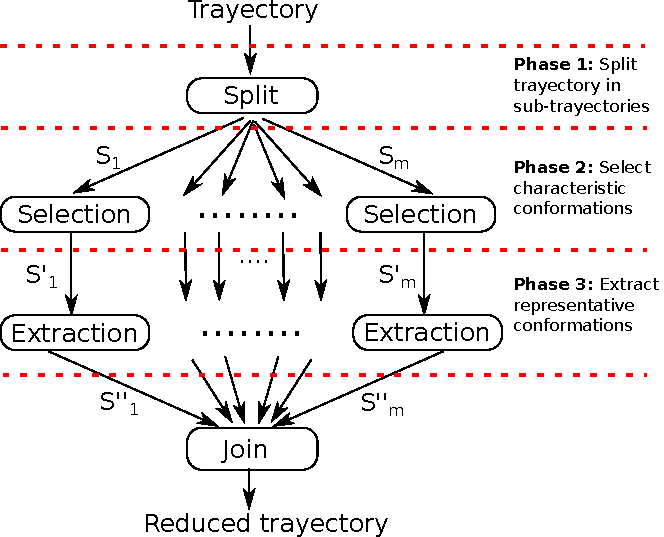
\includegraphics{img/algorithm-flowchart}
\par\end{centering}
\caption{Hola}

\end{figure}

-----------------------------------------------------------

\begin{backmatter}

\section*{Competing interests}

The authors declare that they have no competing interests.

\section*{Author's contributions}

Text for this section \ldots

\section*{Acknowledgements}

Text for this section \ldots


\section*{Figures}

\begin{figure}[h]
\caption{\csentence{Sample figure title.} A short description of the figure content should go here. }

\end{figure}

\begin{figure}[h]
\caption{\csentence{Sample figure title.} Figure legend text. }
\end{figure}


\section*{Tables}

\begin{table}[!h]
\caption{Sample table title. This is where the description of the table should
go.}

\begin{tabular}{cccc}
\hline 
 & B1 & B2 & B3\tabularnewline
\hline 
A1 & 0.1 & 0.2 & 0.3\tabularnewline
A2 & ... & .. & .\tabularnewline
A3 & ... & . & .\tabularnewline
\hline 
\end{tabular}

\end{table}


\section*{Additional Files}

\subsection*{Additional file 1 --- Sample additional file title}

Additional file descriptions text (including details of how to view
the file, if it is in a non-standard format or the file extension).
 This might refer to a multi-page table or a figure.

\subsection*{Additional file 2 -{}-{}- Sample additional file title}

Additional file descriptions text.

\end{backmatter}
\end{document}
\end{document}
